\begin{frame}{Weight Initialization}
	\begin{itemize}
		\item Is initialization really necessary?
		\item What are the impacts of initialization?
		\item A bad initialization may increase convergence time or even make optimization diverge.
		\item How to initialize?
		\begin{itemize}
			\item Zero initialization
			\item Random initialization
		\end{itemize}
	\end{itemize}
	\begin{figure}[H]
		\centering
		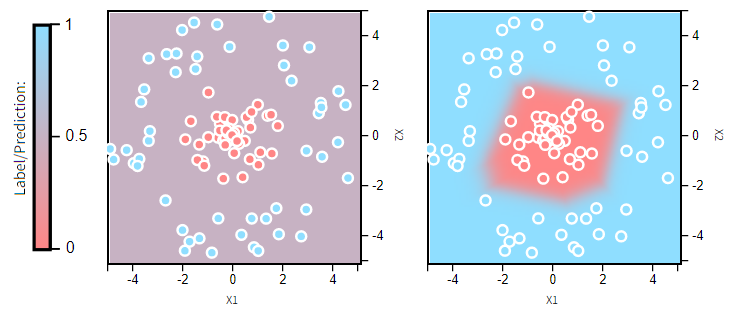
\includegraphics[width=0.65\textwidth]{Figs/wi-crucial.png}
		\caption{The output of a three layer network after about 600 epoch. (left) using a bad\\ initialization method and (right) using an appropriate initialization \cite{katanforoosh-kunin}.}
	\end{figure}
\end{frame}

\begin{frame}{Weight Initialization}
	\begin{block}{Let's review some notations before we continue:}
		\begin{columns}
			\begin{column}{0.4\textwidth}
				\[
				\begin{cases}
					n^{[l]} := \text{layer $l$ neurons number}, \\[0.5em]
					W^{[l]} := \text{layer $l$ weights},\\[0.5em]
					b^{[l]} := \text{layer $l$ biases},\\[0.5em]
					a^{[l]} := \text{layer $l$ outputs}
				\end{cases}
				\]
				\[
				\begin{cases}
					\text{fan}_\text{in}^{[l]} = n^{[l-1]} \quad (\text{layer $l$ number of inputs}),\\[0.6em]
					\text{fan}_\text{out}^{[l]} = n^{[l]} \quad (\text{layer $l$ number of outputs}),\\[0.6em]
					\text{fan}_\text{avg}^{[l]} = \frac{n^{[l-1]} + n^{[l]}}{2}
				\end{cases}
				\]
			\end{column}\hfill
			\begin{column}{0.4\textwidth}
				\begin{figure}[H]
					\centering	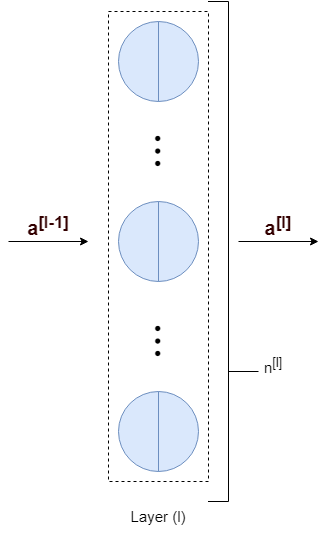
\includegraphics[width=0.65\textwidth]{Figs/notation_review.png}
				\end{figure}
			\end{column}
		\end{columns}
	\end{block}
\end{frame}

\begin{frame}{Weight Initialization: Zero Initialization}
	\begin{block}{Zero Initialization method:}
		\[
		\begin{cases}
			W^{[l]} = \bm{0},\\
			b^{[l]} = \bm{0}
		\end{cases}
		\]
	\end{block}
	\begin{itemize}
		\item[]
		\item[]
		\item Simple but perform very poorly. (why?)
		\item Zero initialization will lead each neuron to learn the same feature
		\item This problem is known as network {\color{red}failing to break symmetry}
		\item In fact any constant initialization suffers from this problem.
	\end{itemize}
\end{frame}

\begin{frame}{Weight Initialization: Zero Initialization}
	\begin{figure}[H]
		\centering
		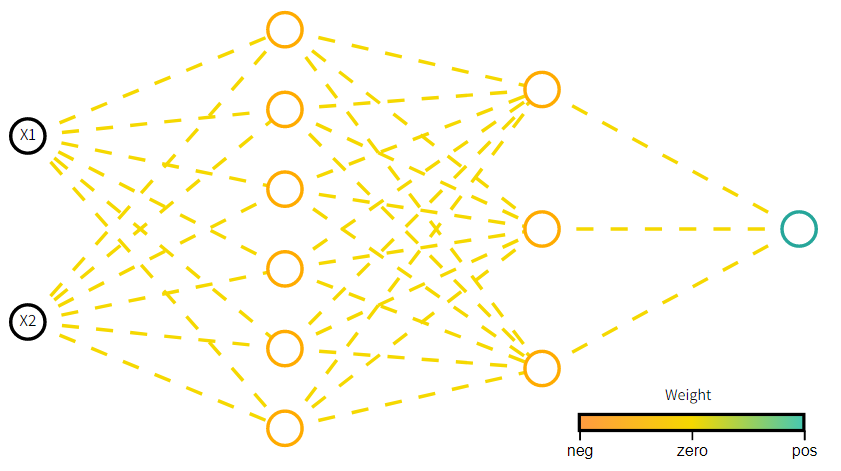
\includegraphics[width=0.65\textwidth]{Figs/zero-init.png}
		\caption{As we can see network has failed to break symmetry. There has been no improvement in weights after about 600 epochs of training \cite{katanforoosh-kunin}.}
	\end{figure}
	\begin{itemize}
		\item We need to break symmetry. How? using randomness.
	\end{itemize}
\end{frame}

\begin{frame}{Weight Initialization: Random Initialization}
	\begin{itemize}
		\item To use randomness in our initialization we can use uniform or normal distribution:
		\medskip
		\item[]\begin{block}{General Uniform Initialization:}
			\[
			\begin{cases}
				W^{[l]} \sim U(-r, +r),\\
				b^{[l]} = 0
			\end{cases}
			\]
		\end{block}
		\item[]\begin{block}{General Normal Initialization:}
			\[
			\begin{cases}
				W^{[l]} \sim \mathcal{N}(\mu=0, \sigma^2),\\
				b^{[l]} = 0
			\end{cases}
			\]
		\end{block}
		\item But this is really crucial to choose $r$ or $\sigma$ properly.
	\end{itemize}
\end{frame}

\begin{frame}{Weight Initialization: Random Initialization}
	\begin{figure}[H]
		\centering
		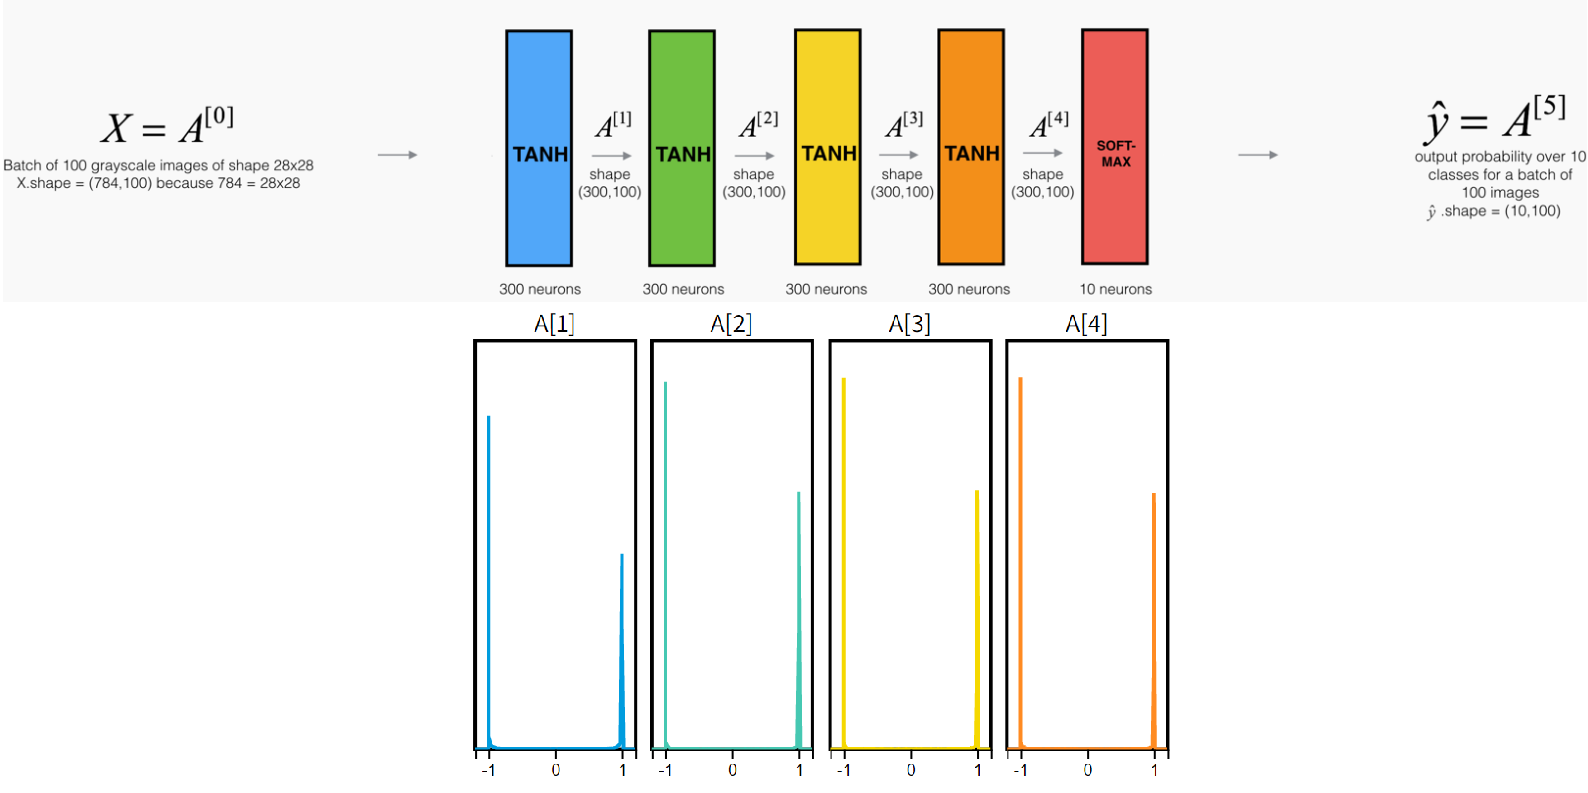
\includegraphics[width=0.9\textwidth]{Figs/normal-init.png}
		\caption{Uniform initialization problem. On the top, you can see the model architecture, and on the bottom, you can see the density of each layer's output. Model has trained on MNIST dataset for 4 epoch. Weights are initialized randomly from $U(\frac{-1}{\sqrt{n^{[l-1]}}}, \frac{1}{\sqrt{n^{[l-1]}}})$ \cite{katanforoosh-kunin}.}
	\end{figure}
\end{frame}

\begin{frame}{Weight Initialization: Random Initialization}
	\begin{itemize}
		\item How to choose $r$ or $\sigma$?
		\item We need to follow these rules:
		\begin{itemize}
			\item keep the mean of the activations zero.
			\item keep the variance of the activations same across every layer.
		\end{itemize}
	\end{itemize}
	\begin{block}{Xavier Initialization:}
		\begin{itemize}
			\item For Uniform distribution use:
			\[
			r = \sqrt{\frac{3}{\text{fan}_\text{avg}}}
			\]
			\item For Normal distribution use:
			\[
			\sigma^2 = \frac{1}{\text{fan}_\text{avg}}
			\]
		\end{itemize}
		{\scriptsize (You can read about why this method works at \cite{katanforoosh-kunin}.)}
	\end{block}
\end{frame}

\begin{frame}{Weight Initialization: Xavier Initialization}
	\begin{itemize}
		\item Xavier initialization works well on \tc{keywords}{Tanh, Logestic or Sigmoid} activation function.
	\end{itemize}
	\begin{figure}[H]
		\centering
		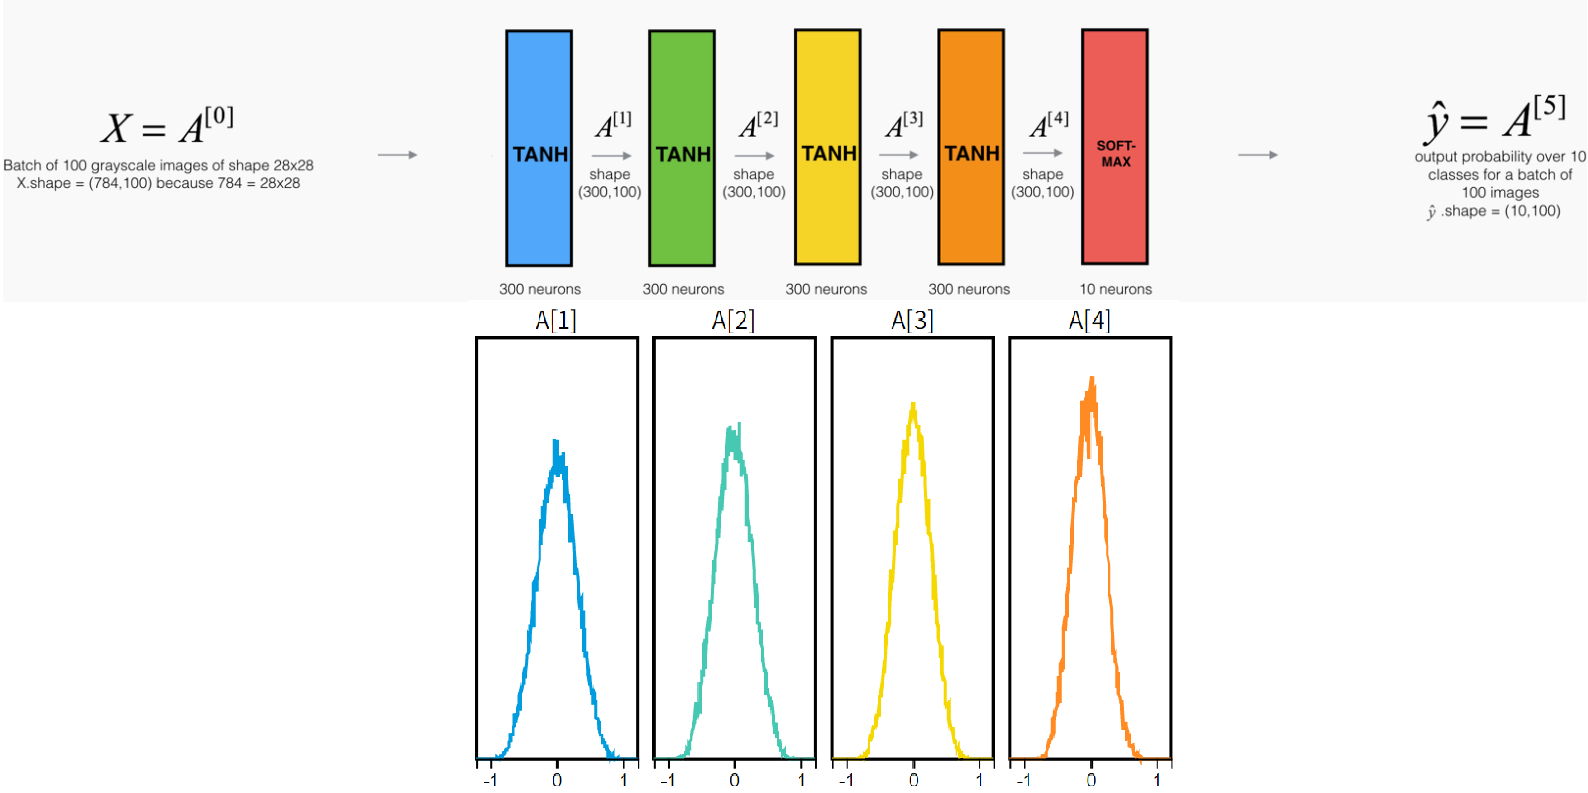
\includegraphics[width=0.9\textwidth]{Figs/xavier-init.png}
		\caption{Vanishing gradient is no longer problem using Xavier initialization. Model has trained on MNIST dataset for 4 epoch. \cite{katanforoosh-kunin}.}
	\end{figure}
\end{frame}

\begin{frame}{Weight Initialization: He Initialization}
	\begin{itemize}
		\item Different method has proposed for different activation functions.
	\end{itemize}
	\begin{block}{He Initialization:}
		\begin{itemize}
			\item For Normal distribution:
			\[
			\sigma^2 = \frac{2}{n^{[l]}}
			\]
			\item For Uniform distribution:
			\[
			r = \sqrt{3\sigma^2}
			\]
		\end{itemize}
	\end{block}
	\begin{itemize}
		\medskip
		\medskip
		\item He initialization works well on \tc{keywords}{ReLU and its variants}.
	\end{itemize}
\end{frame}